\documentclass[a4paper,11pt]{article}
\usepackage[T1]{fontenc}
\usepackage[utf8]{inputenc}
\usepackage{lmodern}
\usepackage[top=0in, bottom=1.25in, left=1.25in, right=1.25in]{geometry}


\usepackage[makeroom]{cancel}
\usepackage[usenames, dvipsnames]{color}
\usepackage{tikz}
\usetikzlibrary{positioning,arrows}
\tikzset{
modal/.style={>=stealth',shorten >=1pt,shorten <=1pt,auto,node distance=1.5cm and 2.5cm,
semithick},
world/.style={circle,draw,minimum size=0.5cm,fill=gray!15},
point/.style={circle,draw,inner sep=0.5mm,fill=black},
reflexive above/.style={->,loop,looseness=7,in=120,out=60},
reflexive below/.style={->,loop,looseness=7,in=240,out=300},
reflexive left/.style={->,loop,looseness=20,in=135,out=225},
reflexive right/.style={->,loop,looseness=20,in=45,out=315}}

\title{}
\author{}

\begin{document}

\maketitle

\section*{Kelewan}
Size: medium\\
Depth of suspicion: 0\\
Tech: 3\\
Attitude: malevolent\\
\\
dW = discovers other world\\
aW = assimilates other world\\
cW = contact other world\\
hW = hide from other world\\
coW = cooperate with other world\\
peW = preemptively strike at other world\\
p = prevails\\
s = survive

\subsection*{$w_0$}

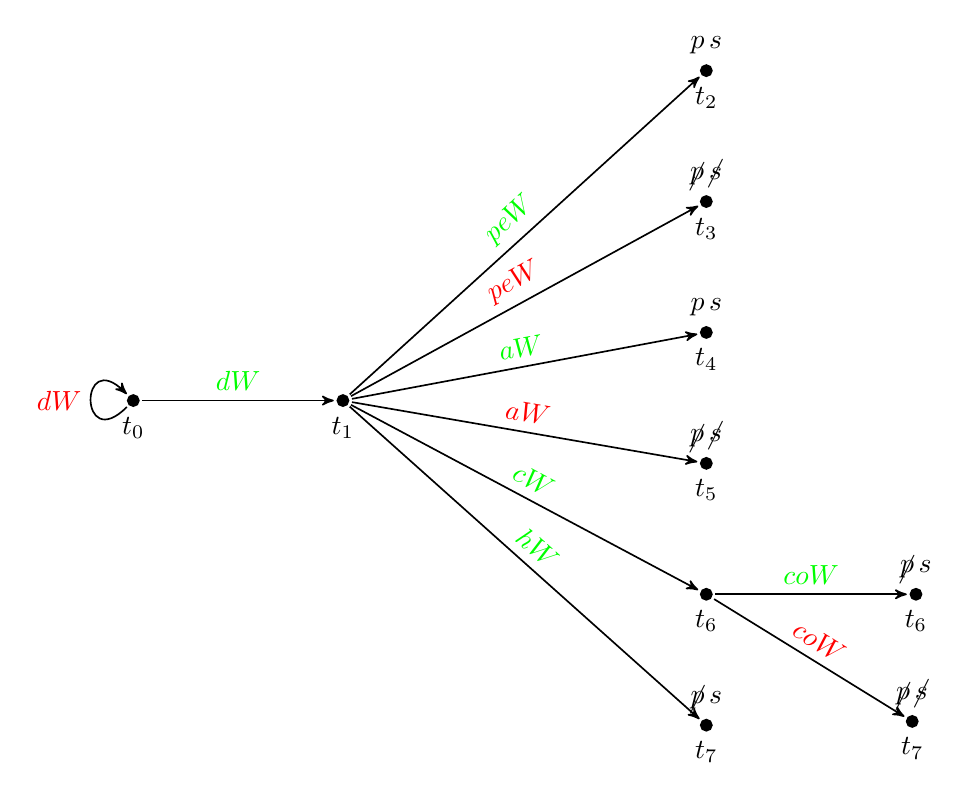
\begin{tikzpicture}[modal]
\node[point] (t0) [label=below:$t_0$] {};

\node[point] (t1) [label=below:$t_1$,right=of t0] {};


\node[point] (t4) [label=below:$t_4$,label=above:$p\,s$,above right=0.75cm and 4.5cm of t1] {};
\node[point] (t3) [label=below:$t_3$,label=above:$\cancel{p}\,\cancel{s}$,above=of t4] {};
\node[point] (t2) [label=below:$t_2$,label=above:$p\,s$,above=of t3] {};
\node[point] (t5) [label=below:$t_5$,label=above:$\cancel{p}\,\cancel{s}$,below=of t4] {};
\node[point] (t6) [label=below:$t_6$,below=of t5] {};
\node[point] (t7) [label=below:$t_7$,label=above:$\cancel{p}\,s$,below=of t6] {};

\node[point] (t8) [label=below:$t_6$,label=above:$\cancel{p}\,s$,right=of t6] {};
\node[point] (t9) [label=below:$t_7$,label=above:$\cancel{p}\,\cancel{s}$,below right=of t6] {};



\path[reflexive left] (t0) edge node [red] {$dW$} (t0) {};
\path[->] (t0) edge node [green, sloped] {$dW$} (t1);

\path[->] (t1) edge node [green, sloped] {$peW$} (t2);
\path[->] (t1) edge node [red, sloped] {$peW$} (t3);
\path[->] (t1) edge node [green, sloped] {$aW$} (t4);
\path[->] (t1) edge node [red, sloped] {$aW$} (t5);
\path[->] (t1) edge node [green, sloped] {$cW$} (t6);
\path[->] (t1) edge node [green, sloped] {$hW$} (t7);

\path[->] (t6) edge node [green, sloped] {$coW$} (t8);
\path[->] (t6) edge node [red, sloped] {$coW$} (t9);

\end{tikzpicture}


\subsection*{$b_0$}
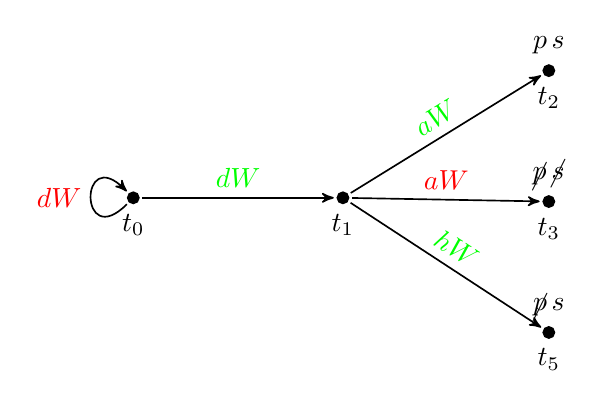
\begin{tikzpicture}[modal]
\node[point] (t0) [label=below:$t_0$] {};

\node[point] (t1) [label=below:$t_1$,right=of t0] {};
\node[point] (t2) [label=below:$t_2$,label=above:$p\,s$,above right=of t1] {};

\node[point] (t3) [label=below:$t_3$,label=above:$\cancel{p}\,\cancel{s}$,below=of t2] {};
\node[point] (t5) [label=below:$t_5$,label=above:$\cancel{p}\,s$,below=of t3] {};

\path[reflexive left] (t0) edge node [red] {$dW$} (t0) {};
\path[->] (t0) edge node [green, sloped] {$dW$} (t1);

\path[->] (t1) edge node [green, sloped] {$aW$} (t2);
\path[->] (t1) edge node [red, sloped] {$aW$} (t3);
\path[->] (t1) edge node [green, sloped] {$hW$} (t5);
\end{tikzpicture}


\subsection*{$g_0$}
\begin{tikzpicture}[modal]
\node[point] (t0) [label=below:$t_0$] {};

\node[point] (t1) [label=below:$t_1$,right=of t0] {};
\node[point] (t2) [label=below:$t_2$,label=above:$p\,s$,above right=of t1] {};

\node[point] (t5) [label=below:$t_5$,label=above:$\cancel{p}\,s$,below=of t3] {};

\path[->] (t0) edge node [green, sloped] {$dW$} (t1);

\path[->] (t1) edge node [green, sloped] {$aW$} (t2);
\path[->] (t1) edge node [green, sloped] {$hW$} (t5);
\end{tikzpicture}

\subsection*{$i_0$}
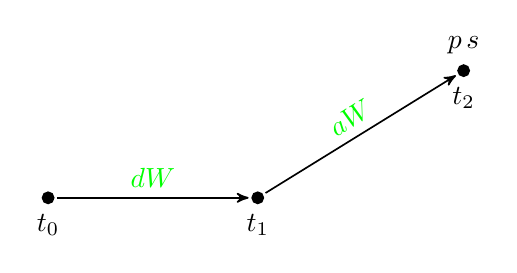
\begin{tikzpicture}[modal]
\node[point] (t0) [label=below:$t_0$] {};

\node[point] (t1) [label=below:$t_1$,right=of t0] {};
\node[point] (t2) [label=below:$t_2$,label=above:$p\,s$,above right=of t1] {};

\path[->] (t0) edge node [green, sloped] {$dW$} (t1);

\path[->] (t1) edge node [green, sloped] {$aW$} (t2);
\end{tikzpicture}

\section*{$i_1$}
\begin{tikzpicture}[modal]
\node[point] (t0) [label=below:$t_0$] {};
\node[point] (t1) [label=below:$t_1$,right=of t0] {};
\node[point] (t5) [label=below:$t_5$,label=above:$\cancel{p}\,s$,below=of t3] {};

\path[->] (t0) edge node [green, sloped] {$dW$} (t1);
\path[->] (t1) edge node [green, sloped] {$hW$} (t5);
\end{tikzpicture}

\subsection*{If Kelewan were benevolent}

\subsection*{$b_0$}

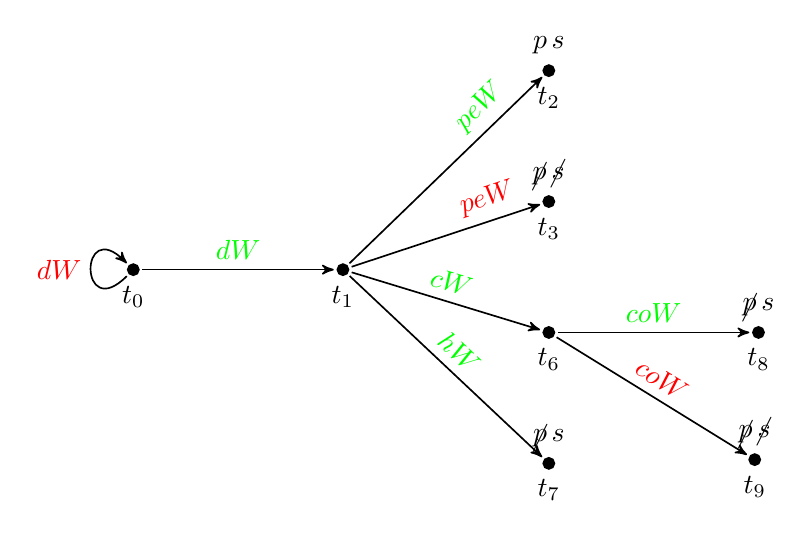
\begin{tikzpicture}[modal]
\node[point] (t0) [label=below:$t_0$] {};

\node[point] (t1) [label=below:$t_1$,right=of t0] {};


\node[point] (t3) [label=below:$t_3$,label=above:$\cancel{p}\,\cancel{s}$,above right=0.75cm and 2.5cm of t1] {};
\node[point] (t2) [label=below:$t_2$,label=above:$p\,s$,above=of t3] {};
\node[point] (t6) [label=below:$t_6$,below=of t3] {};
\node[point] (t7) [label=below:$t_7$,label=above:$\cancel{p}\,s$,below=of t6] {};

\node[point] (t8) [label=below:$t_8$,label=above:$\cancel{p}\,s$,right=of t6] {};
\node[point] (t9) [label=below:$t_9$,label=above:$\cancel{p}\,\cancel{s}$,below right=of t6] {};



\path[reflexive left] (t0) edge node [red] {$dW$} (t0) {};
\path[->] (t0) edge node [green, sloped] {$dW$} (t1);

\path[->] (t1) edge node [green, sloped, near end] {$peW$} (t2);
\path[->] (t1) edge node [red, sloped, near end] {$peW$} (t3);
\path[->] (t1) edge node [green, sloped] {$cW$} (t6);
\path[->] (t1) edge node [green, sloped] {$hW$} (t7);

\path[->] (t6) edge node [green, sloped] {$coW$} (t8);
\path[->] (t6) edge node [red, sloped] {$coW$} (t9);
\end{tikzpicture}

\subsection*{$g_0$}
g(coW) || g(s)
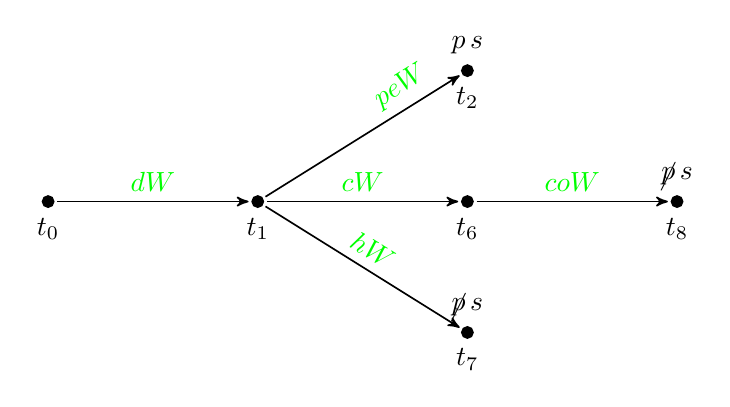
\begin{tikzpicture}[modal]
\node[point] (t0) [label=below:$t_0$] {};

\node[point] (t1) [label=below:$t_1$,right=of t0] {};

\node[point] (t6) [label=below:$t_6$,right=of t1] {};
\node[point] (t2) [label=below:$t_2$,label=above:$p\,s$,above=of t6] {};
\node[point] (t7) [label=below:$t_7$,label=above:$\cancel{p}\,s$,below=of t6] {};

\node[point] (t8) [label=below:$t_8$,label=above:$\cancel{p}\,s$,right=of t6] {};


\path[->] (t0) edge node [green, sloped] {$dW$} (t1);

\path[->] (t1) edge node [green, sloped, near end] {$peW$} (t2);
\path[->] (t1) edge node [green, sloped] {$cW$} (t6);
\path[->] (t1) edge node [green, sloped] {$hW$} (t7);

\path[->] (t6) edge node [green, sloped] {$coW$} (t8);
\end{tikzpicture}

\subsection*{$i_0$}
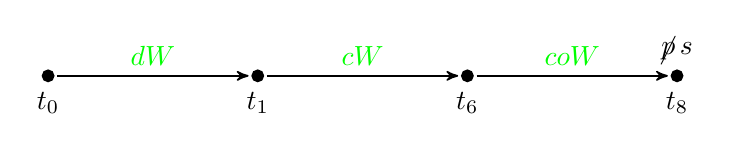
\begin{tikzpicture}[modal]
\node[point] (t0) [label=below:$t_0$] {};

\node[point] (t1) [label=below:$t_1$,right=of t0] {};

\node[point] (t6) [label=below:$t_6$,right=of t1] {};

\node[point] (t8) [label=below:$t_8$,label=above:$\cancel{p}\,s$,right=of t6] {};



\path[->] (t0) edge node [green, sloped] {$dW$} (t1);

\path[->] (t1) edge node [green, sloped] {$cW$} (t6);

\path[->] (t6) edge node [green, sloped] {$coW$} (t8);
\end{tikzpicture}

\subsection*{$i_1$}
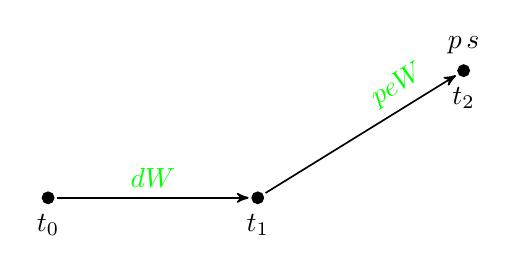
\begin{tikzpicture}[modal]
\node[point] (t0) [label=below:$t_0$] {};

\node[point] (t1) [label=below:$t_1$,right=of t0] {};

\node[point] (t2) [label=below:$t_2$,label=above:$p\,s$,above right=of t1] {};

\path[->] (t0) edge node [green, sloped] {$dW$} (t1);

\path[->] (t1) edge node [green, sloped, near end] {$peW$} (t2);
\end{tikzpicture}

\subsection*{$i_2$}
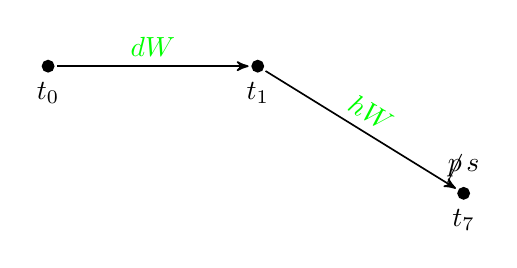
\begin{tikzpicture}[modal]
\node[point] (t0) [label=below:$t_0$] {};

\node[point] (t1) [label=below:$t_1$,right=of t0] {};

\node[point] (t7) [label=below:$t_7$,label=above:$\cancel{p}\,s$,below right=of t1] {};

\path[->] (t0) edge node [green, sloped] {$dW$} (t1);

\path[->] (t1) edge node [green, sloped] {$hW$} (t7);
\end{tikzpicture}

\subsection*{Chain of suspicion}
h = go into hiding

\begin{tikzpicture}[modal]
\node[point] (t0) [label=below:$s$] {};

\node[point] (t1) [label=below:$d_1$,label=above:$b$,above right=of t0] {};
\node[point] (t2) [label=below:$d_1$,label=above:$m$,below right=of t0] {};

\node[point] (t3) [label=below:$d_2$,label=above:$wb$,above right=of t1] {};
\node[point] (t4) [label=below:$d_2$,label=above:$wm$,below right=of t1] {};

\node[point] (t5) [label=below:$d_3$,label=above:$b$,above right=of t3] {};
\node[point] (t6) [label=below:$d_3$,label=above:$m$,below right=of t3] {};

\node[point] (t7) [label=below:$d_4$,label=above:$wb$,above right=of t5] {};
\node[point] (t8) [label=below:$d_4$,label=above:$wm$,below right=of t5] {};

\path[->] (t0) edge node [green, sloped] {} (t1);
\path[->] (t0) edge node [green, sloped] {} (t2);

\path[->] (t1) edge node [green, sloped] {} (t3);
\path[->] (t1) edge node [green, sloped] {} (t4);

\path[->] (t3) edge node [green, sloped] {} (t5);
\path[->] (t3) edge node [green, sloped] {} (t6);

\path[->] (t5) edge node [green, sloped] {} (t7);
\path[->] (t5) edge node [green, sloped] {} (t8);
\end{tikzpicture}

\end{document}
